\documentclass[conference]{IEEEtran}
% Compile on Overleaf (pdfLaTeX + BibTeX). IEEEtran.cls is built into Overleaf.
\IEEEoverridecommandlockouts
\usepackage{cite}
\usepackage{amsmath,amssymb}
\usepackage{graphicx}
\usepackage{booktabs}
\usepackage{multirow}
\usepackage{url}
\usepackage[hidelinks]{hyperref}
\graphicspath{{figures/}}

\begin{document}

\title{Leakage-Aware Evaluation of Federated Intrusion Detection under Poisoning, Evasion and LLM-Planned Attacks}

\author{\IEEEauthorblockN{Vinit Soni}
\IEEEauthorblockA{\textit{School of Computer Science Engineering and Technology} \\
\textit{Bennett University}\\
Greater Noida, India \\
[email]}
% Add the project guide as a second author block here if required:
% \and
% \IEEEauthorblockN{[Guide name]}
% \IEEEauthorblockA{...}
}

\maketitle

\begin{abstract}
Federated intrusion detection for IoT networks is commonly reported with F1-scores of 0.92--0.99 on CICIoT2023. We re-examine it under a stricter protocol and against three threats in one pipeline: model-update poisoning, inference-time evasion and attacks planned by large language models (LLMs).
An audit of the local CICIoT2023 release found 55.0\,\% exact duplicate rows and 30.6\,\% of rows that share their feature vector with another class. We therefore use a file- and time-aware, de-duplicated split.
Under this split, test macro-F1 is $0.687\pm0.005$ (8 classes) for a multilayer perceptron, within 0.01--0.03 of the dataset authors' own benchmark, while recent federated studies on balanced or random samples report 0.92--0.99. At a validation-calibrated 1\,\% benign false-positive rate (FPR), the detectors still find 83--86\,\% of attack windows.
Federated averaging costs 0.6--2.5 points of detection with IID or moderately skewed clients, but strong label skew (Dirichlet $\alpha=0.1$) breaks both FedAvg and FedProx.
Two malicious clients out of ten collapse FedAvg. Coordinate-wise median and trimmed mean neutralise the attacks with IID clients, but only partially with non-IID clients.
A label-only black-box attacker that can only pad, slow down and re-TTL its own packets evades the deployable 1\,\%-FPR rule for 24--49\,\% of detected windows. Two rounds of adversarial training reduce this to 8--17\,\%.
On GridStratLLM, LLM-planned attacks are detected across planning LLMs (leave-one-LLM-out AUC 0.90--1.00), even without the ARP signature.
A Flower deployment across two Azure virtual machines and a laptop reproduces the simulator to four decimals.
\end{abstract}

\begin{IEEEkeywords}
intrusion detection, federated learning, IoT security, model poisoning, adversarial evasion, data leakage, LLM-coordinated attacks
\end{IEEEkeywords}

\section{Introduction}
Machine-learning network intrusion detection systems (NIDS) for the Internet of Things are routinely reported with near-perfect scores. On CICIoT2023~\cite{neto2023ciciot}, recent federated studies report 8-class F1 of 0.92--0.95~\cite{bilal2026dataset} and binary F1 of 0.99~\cite{nayak2026byzantine}.

Three facts make these numbers hard to act on:
\begin{enumerate}
\item \textbf{Leakage.} IoT traffic datasets contain many duplicate and near-duplicate windows, and random splits let them appear in both training and test data~\cite{arp2022dos}.
\item \textbf{Two attack surfaces.} Federated learning (FL)~\cite{mcmahan2017fedavg} opens the model to poisoning by malicious clients~\cite{bagdasaryan2020backdoor}, and the deployed model to evasion by attackers who shape their own traffic~\cite{apruzzese2022realistic}. The two are rarely studied together.
\item \textbf{LLM-planned attacks.} Attacks are beginning to be planned by LLM agents~\cite{kellerer2026gridstrat}, and it is not known whether their network signatures depend on the planner.
\end{enumerate}

This paper evaluates all of these in one reproducible pipeline. It makes the following contributions:
\begin{itemize}
\item A provenance and leakage audit of the local CICIoT2023 release, and a file- and time-aware, de-duplicated split. We show that our multi-class results agree with the dataset authors' benchmark, and we explain the gap to recent federated studies by protocol differences (Section~\ref{sec:lit}).
\item An operating-point view of detection: thresholds fitted on validation for 5\,\% and 1\,\% benign FPR. We show that the deployable threshold is also the most evadable one.
\item FedAvg and FedProx under IID and Dirichlet label skew for 2, 8 and 34 classes. Poisoning is evaluated with three robust aggregators and a malicious-fraction sweep, and compared with Nayak and Reddy~\cite{nayak2026byzantine}.
\item A realisable label-only evasion attack with adversarial training, evaluated on the same detectors.
\item A leave-one-LLM-out evaluation on GridStratLLM~\cite{kellerer2026gridstratdata}, with and without the ARP signature.
\item A Flower deployment across Azure and a laptop that reproduces the simulator, and an authenticated model endpoint.
\end{itemize}

\section{Related Work and Comparison}\label{sec:lit}
\textbf{Dataset benchmark.} Neto et al.~\cite{neto2023ciciot} shuffle CICIoT2023 and split it at random 80/20. They report accuracy above 98\,\% for random forest (RF) and a deep neural network (DNN), but macro-F1 of only 0.719 / 0.697 for 8 classes and 0.714 / 0.672 for 34 classes. The remaining errors lie among Benign, Recon, Spoofing, Web and Brute force.

\textbf{Federated IDS.} Bilal et al.~\cite{bilal2026dataset} compare FedAvg, FedProx and FedNova with LSTM and Transformer backbones on three IoT datasets. CIC-IoT2023 is split into 10 device-group clients. They report 8-class F1 of 0.920--0.952 from single runs with a roughly balanced test set, and find that FedProx and FedNova gain 1--2 points.

\textbf{Poisoning.} Nayak and Reddy~\cite{nayak2026byzantine} compare five aggregators on a balanced binary sample of CICIoT2023 with 20 clients ($\alpha=0.3$), over 641 runs with five seeds and corrected significance tests. FedAvg collapses under 30\,\% sign-flipping. The median and trimmed mean break at 20\,\%, while multi-Krum and FLTrust hold. Client-level differential privacy destroyed utility at every budget they tested.

\textbf{LLMs and attacks.} Kampourakis et al.~\cite{kampourakis2026k2d} use LLMs to \emph{generate} synthetic AWID3 traffic (F1 up to 0.956 when transferred to real data). GridStratLLM~\cite{kellerer2026gridstrat} instead records attacks \emph{planned} by LLMs on a hardware-in-the-loop smart-grid testbed.

\textbf{Methods.} Robust aggregation by median and trimmed mean follows~\cite{yin2018byzantine}, targeted poisoning with boosting follows~\cite{bagdasaryan2020backdoor,sun2019backdoor}, and Dirichlet partitions follow~\cite{hsu2019noniid}. The problem-space constraints on evasion follow~\cite{apruzzese2022realistic,pierazzi2020problemspace}.

Table~\ref{tab:scope} summarises the scope of each study. No prior study combines a leakage-aware protocol, a fixed operating point, poisoning, evasion and LLM-planned attacks.

\begin{table}[t]
\caption{Scope of related studies and this work}\label{tab:scope}
\centering\footnotesize
\setlength{\tabcolsep}{2.5pt}
\begin{tabular}{@{}lccccc@{}}
\toprule
 & \cite{neto2023ciciot} & \cite{bilal2026dataset} & \cite{nayak2026byzantine} & \cite{kampourakis2026k2d} & Ours \\
\midrule
Leakage-aware split & -- & -- & -- & -- & \checkmark \\
Fixed benign FPR & -- & -- & -- & -- & \checkmark \\
Federated training & -- & \checkmark & \checkmark & -- & \checkmark \\
Real FL deployment & -- & -- & -- & -- & \checkmark \\
Poisoning + robust agg. & -- & -- & \checkmark & -- & \checkmark \\
Evasion (+ defence) & -- & -- & -- & -- & \checkmark \\
LLM-related attacks & -- & -- & -- & data gen. & planned \\
Multi-seed & -- & -- & \checkmark & -- & \checkmark \\
\bottomrule
\end{tabular}
\end{table}

\section{Data and Leakage-Aware Protocol}
\textbf{CICIoT2023 audit.} The local release has 309 CSV files with 46,776,700 windows and 39 features, and no label column. Labels come from folder names and were checked against traffic content. The audit found:
\begin{itemize}
\item 55.0\,\% exact duplicate rows;
\item 30.6\,\% of rows sharing their feature vector with a row of another class, mostly DDoS-$X$ against DoS-$X$;
\item six features that encode the per-family extraction window (100 or 10 packets);
\item rows that are time-ordered within files.
\end{itemize}

\textbf{Split.} Classes with three or more capture files are split by file. The 17 classes with one or two files are split into purged 70/15/15 time blocks. Rows are de-duplicated within each split and capped per class, giving 664,187 training, 132,923 validation and 253,328 test windows.

We also score the whole test pool (8,980,013 windows at the natural class prior). Because 12.2\,\% of test vectors also occur in the training pool, we report an ``unseen'' subset as well. Preprocessing (median imputation, signed log, standardisation) is fitted on training data only and uses the 33 window-invariant features.

\textbf{GridStratLLM.} The dataset has 436 attack sessions planned by four LLMs and 1.75\,h of normal operation. We use 10\,s windows with a 20\,s guard band, identity-free features, leave-one-LLM-out folds, and a time-split normal hold-out (0.70\,h).

\section{Methods and Threat Models}
Fig.~\ref{fig:arch} shows the pipeline.

\begin{figure*}[t]
\centering
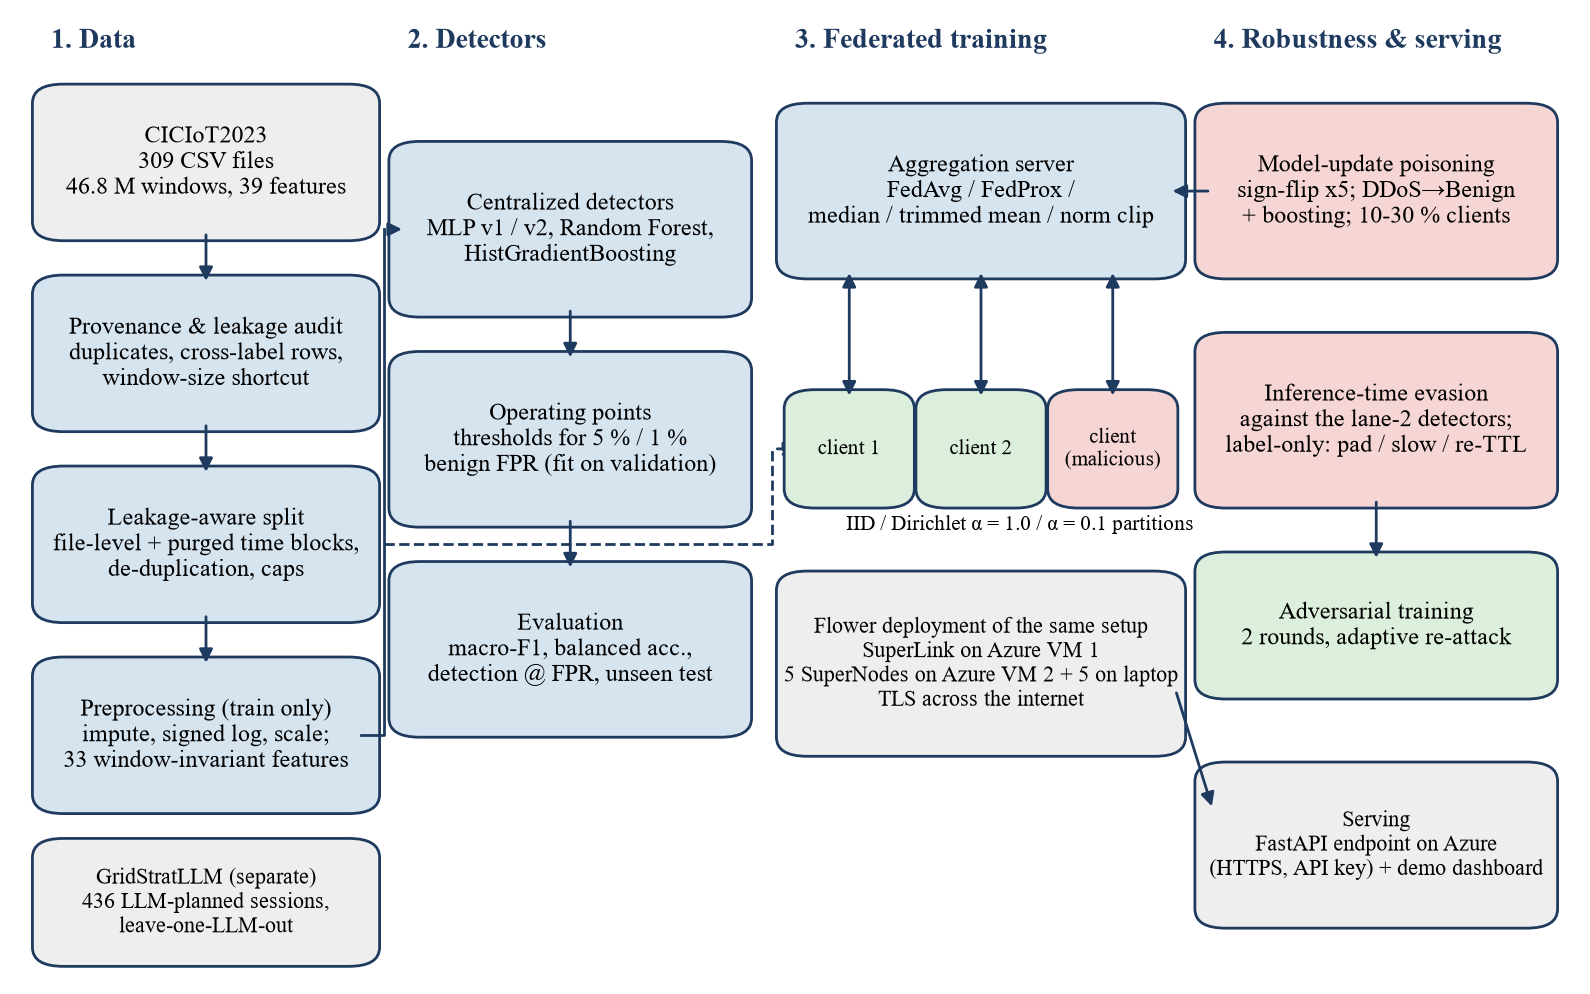
\includegraphics[width=0.86\textwidth]{doc_architecture.png}
\caption{System architecture: leakage-aware data preparation, calibrated detectors, federated training (simulated, and deployed with Flower across Azure and a laptop), and the attacks, defence and serving.}
\label{fig:arch}
\end{figure*}

\textbf{Detectors.} We use three models:
\begin{itemize}
\item \emph{v1 MLP:} 33-128-64-$K$ (13,128 parameters for $K=8$), Adam, square-root inverse class weights, early stopping on validation macro-F1.
\item \emph{v2 MLP:} 256-128 hidden units with dropout 0.1, selected by a 24-configuration search on validation with three seeds.
\item \emph{Tree baselines:} RF and HistGradientBoosting (HGB).
\end{itemize}
The attack score is $1-P(\text{Benign})$. Thresholds are set on validation so that at most 5\,\% or 1\,\% of benign windows are flagged; above the threshold, the most probable attack class is assigned.

\textbf{Federated learning.} The simulator uses 10 clients with full participation, 30 rounds and one local epoch. Partitions are IID or Dirichlet with $\alpha\in\{1.0, 0.1\}$, and the algorithms are FedAvg~\cite{mcmahan2017fedavg} and FedProx~\cite{li2020fedprox} ($\mu=0.01$). The same model and partitions also run as Flower processes: the server on one Azure VM, five clients on a second VM and five on a laptop, over TLS.

\textbf{Poisoning.} Two of ten clients are malicious by default, and the fraction is swept from 10\,\% to 30\,\%. Two attacks are used:
\begin{itemize}
\item \emph{Sign-flip $\times5$:} the malicious update is negated and scaled by five.
\item \emph{DDoS$\rightarrow$Benign:} the client relabels its DDoS rows as Benign and boosts its update.
\end{itemize}
The defences are coordinate-wise median, trimmed mean ($\beta=0.2$) and norm clipping to the median update norm~\cite{yin2018byzantine}.

\textbf{Evasion.} The attacker is black-box, sees labels only, and has at most 112 queries per window. It may change only its own packets:
\begin{itemize}
\item pad them up to the MTU (1514\,B);
\item slow down by a factor $r\ge0.1$;
\item set the TTL to a benign quantile.
\end{itemize}
Every success is re-checked against these constraints and re-queried; there were zero violations. The evasion rate is the share of detected windows turned Benign.

\textbf{Adversarial training.} Each round, successful adversarial training windows are added with their true labels, the model is retrained, and it is re-attacked adaptively on a fixed test sample. We run two rounds.

\section{Results}
All values are test-set results. Where three seeds were run, we give the mean $\pm$ the standard deviation.

\subsection{Detection, and comparison with prior work}
Table~\ref{tab:det} and Fig.~\ref{fig:lit} put our results next to those reported for CICIoT2023.

\textbf{Agreement with the dataset authors.} Our 8-class macro-F1 (MLP 0.687, RF 0.709) is within 0.01--0.03 of Neto et al.'s own benchmark, and the hard classes are the same. The 0.92--0.99 results in~\cite{bilal2026dataset,nayak2026byzantine} come from balanced or random samples, which hide the benign class. Their split files are not public, so the effect of each factor cannot be isolated.

\textbf{Binary results depend on the class prior.} Our binary MLP scores 0.750 on the de-duplicated, capped test set, but 0.920 on the whole test pool at the natural prior, close to Neto et al.'s DNN (0.940).

\textbf{Accuracy and confusion.} Our 8-class accuracy is 0.807 (MLP) and 0.828 (RF), against 0.994 in~\cite{neto2023ciciot}. Fig.~\ref{fig:cm} shows where the errors lie. DDoS and DoS, the two largest classes, are confused with each other (18--22\,\% for the MLP). Most of the 30.6\,\% of raw rows that share their feature vector with another class are DDoS-$X$/DoS-$X$ pairs. Web and Brute force fall mostly into Recon. Binary accuracy on the whole test pool is 0.990 (MLP), close to the 0.997 reported in~\cite{neto2023ciciot}.

\begin{figure*}[t]
\centering
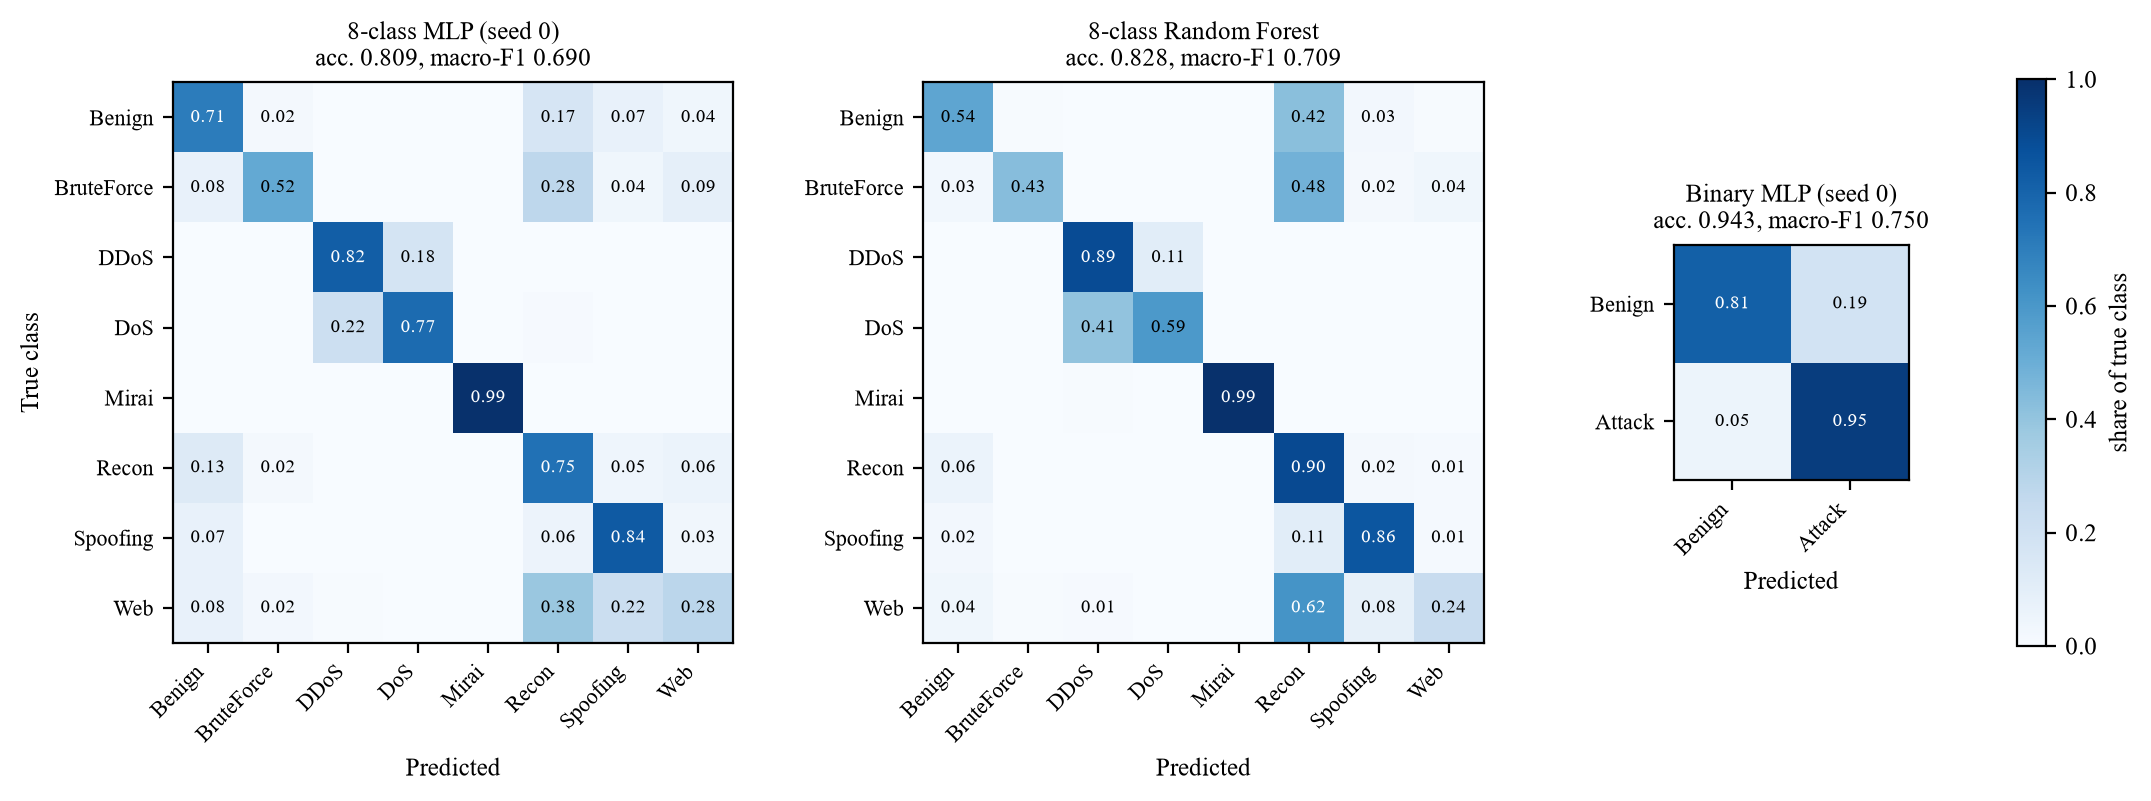
\includegraphics[width=0.92\textwidth]{doc_confusion.png}
\caption{Row-normalised test confusion matrices: 8-class MLP (seed 0), 8-class RF, and binary MLP (seed 0).}
\label{fig:cm}
\end{figure*}

\textbf{Accuracy hides false alarms.} At argmax, every model flags 19--29\,\% of benign windows. At the 1\,\% validation threshold, the achieved test FPR is 0.7--1.3\,\%, and attack detection is 0.852 / 0.846 / 0.833 for the v2 MLP and 0.862 / 0.849 / 0.861 for HGB (8-class / 34-class / binary).

\begin{table}[t]
\caption{CICIoT2023 F1 by evaluation protocol (macro-F1 for multi-class)}\label{tab:det}
\centering\footnotesize
\setlength{\tabcolsep}{3pt}
\begin{tabular}{@{}llll@{}}
\toprule
Study & Task, model & Protocol & F1 \\
\midrule
\cite{neto2023ciciot} & 8-cl., RF / DNN & random 80/20 & 0.719 / 0.697 \\
\cite{neto2023ciciot} & 2-cl., RF / DNN & random 80/20 & 0.965 / 0.940 \\
\cite{bilal2026dataset} & 8-cl., FL & balanced test & 0.920--0.952 \\
\cite{nayak2026byzantine} & 2-cl., FL & balanced sample & 0.989--0.990 \\
\midrule
Ours & 8-cl., MLP / RF & file/time, dedup. & 0.687 / 0.709 \\
Ours & 34-cl., MLP v2 / RF & file/time, dedup. & 0.574 / 0.591 \\
Ours & 2-cl., MLP & file/time, dedup. & 0.750 \\
Ours & 2-cl., MLP & natural prior pool & 0.920 \\
Ours & 8-cl., FedAvg IID & file/time, dedup. & 0.668 \\
\bottomrule
\end{tabular}
\end{table}

\begin{figure}[t]
\centering
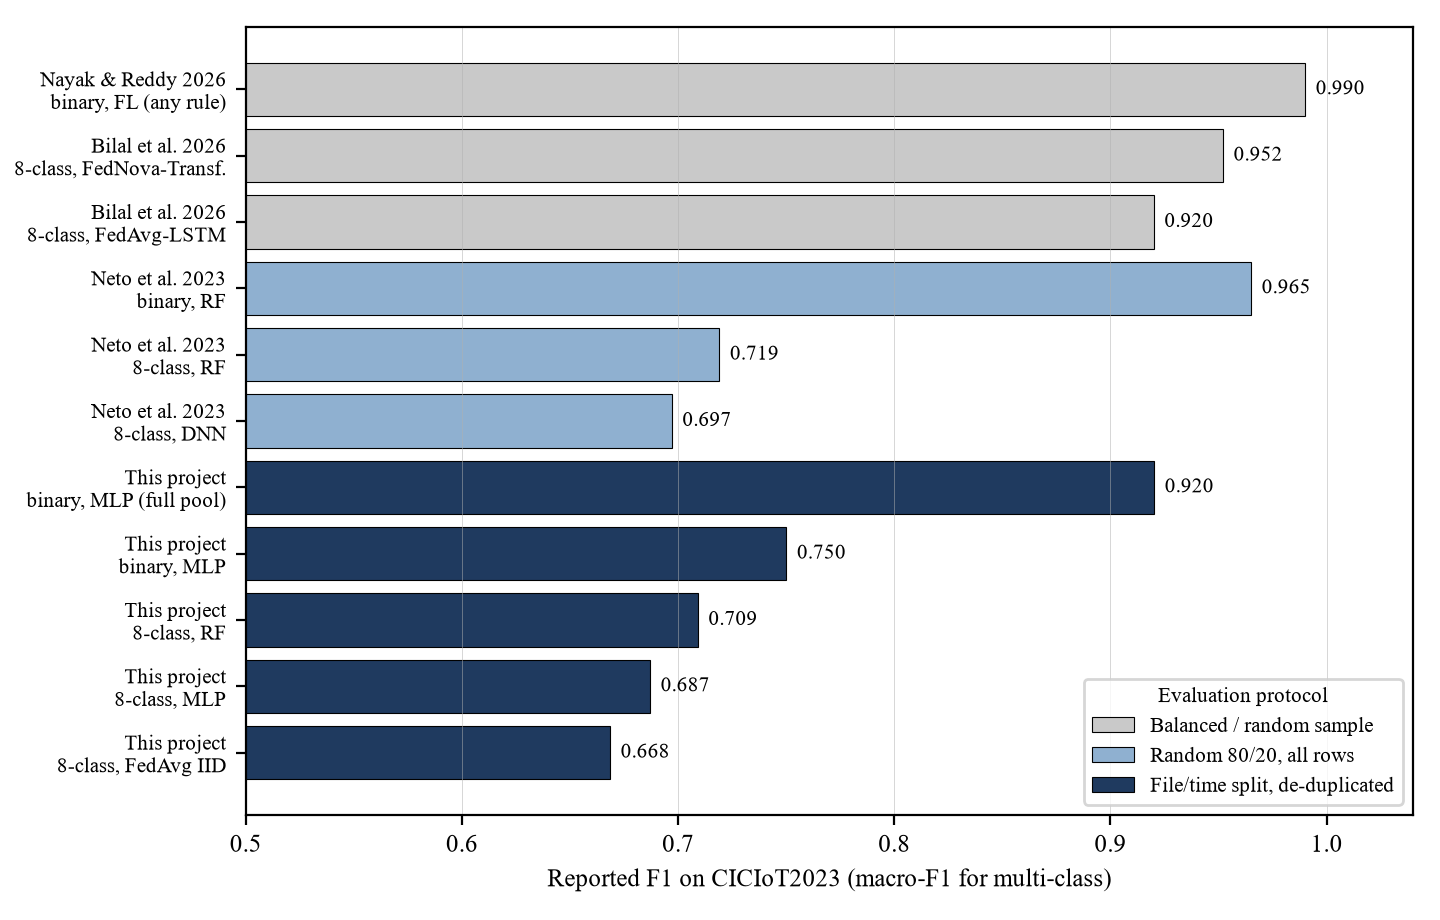
\includegraphics[width=\columnwidth]{doc_lit_comparison.png}
\caption{Reported CICIoT2023 F1 in prior work and in this work, coloured by evaluation protocol.}
\label{fig:lit}
\end{figure}

\subsection{Federated learning}
Table~\ref{tab:fl} gives the federated results.

\textbf{Mild heterogeneity.} With IID or $\alpha=1.0$ clients, FL is 0.02--0.04 macro-F1 below centralised training, or 0.6--2.5 points of detection at 1\,\% FPR. This agrees with~\cite{bilal2026dataset}.

\textbf{FedProx.} FedProx's change is within one standard deviation. Bilal et al. report a 1-point gain.

\textbf{Strong label skew.} With $\alpha=0.1$, training breaks in all tasks: the benign FPR rises to about 0.6, with large seed variance. Re-running for 60 rounds showed this is not under-training: round 30 of each 60-round run equals the 30-round run, and 8-class $\alpha=0.1$ stays at 0.31--0.51.

\textbf{Realism variants (v2 MLP, one seed).}
\begin{itemize}
\item Two local epochs give up to +1.4 points at the same communication cost.
\item Half participation halves communication at a cost of at most 0.4 points.
\item 20 clients cost up to 2.7 points.
\end{itemize}

\textbf{Real deployment.} The Flower deployment across Azure and the laptop reached test macro-F1 0.6692, identical to the simulator with the same seed and partition. It was about 6$\times$ slower because of CPU clients and network round trips.

\begin{table}[t]
\caption{Federated test macro-F1 (3 seeds, 10 clients, 30 rounds)}\label{tab:fl}
\centering\footnotesize
\setlength{\tabcolsep}{3pt}
\begin{tabular}{@{}llll@{}}
\toprule
Setting & 8-class & 34-class & binary \\
\midrule
Centralised & $0.687\pm.005$ & $0.556\pm.027$ & $0.750\pm.004$ \\
FedAvg IID & $0.668\pm.001$ & $0.520\pm.001$ & $0.741\pm.000$ \\
FedProx IID & $0.667\pm.001$ & $0.512\pm.003$ & $0.740\pm.001$ \\
FedAvg $\alpha{=}1.0$ & $0.667\pm.008$ & $0.514\pm.007$ & $0.758\pm.001$ \\
FedAvg $\alpha{=}0.1$ & $0.423\pm.107$ & $0.425\pm.027$ & $0.632\pm.137$ \\
FedProx $\alpha{=}0.1$ & $0.469\pm.106$ & $0.426\pm.026$ & $0.640\pm.128$ \\
\bottomrule
\end{tabular}
\end{table}

\subsection{Model-update poisoning}
Table~\ref{tab:pois} gives the poisoning results with IID clients.

\textbf{FedAvg.} Two malicious clients defeat FedAvg in every task. Sign-flipping collapses it to a single class (macro-F1 0.003--0.038). The targeted attack hides 23--62\,\% of DDoS windows as Benign, but it is not stealthy: macro-F1 falls and the benign FPR rises.

\textbf{Robust rules.} With IID clients, all three robust rules keep macro-F1 within 0.016 of clean and DDoS$\rightarrow$Benign at or below 0.3\,\%. Their clean cost is at most 0.001, and their runtime cost is negligible (92--94\,s per run).

\textbf{Non-IID clients.} With $\alpha=1.0$ (one seed), protection is partial: sign-flipping raises the 8-class benign FPR from 0.31--0.33 to 0.42--0.50.

\textbf{Fraction sweep.} At 30\,\% malicious clients, the trimmed mean (which trims two values per side) fails (8-class 0.477), while the median holds (0.665).

\textbf{Comparison with~\cite{nayak2026byzantine}.} Nayak and Reddy observe the same pattern: FedAvg collapses, and coordinate-wise rules hold only within their assumptions. Their rules break earlier (at 20\,\%), which is consistent with their stronger client skew ($\alpha=0.3$, 20 clients). We did not evaluate multi-Krum or FLTrust, the strongest rules in their study.

\begin{table}[t]
\caption{Test macro-F1 under poisoning, 2 of 10 clients malicious, IID (3 seeds). DDoS$\rightarrow$B in brackets.}\label{tab:pois}
\centering\footnotesize
\setlength{\tabcolsep}{2.5pt}
\begin{tabular}{@{}lllll@{}}
\toprule
Attack & Aggregator & 8-class & 34-class & binary \\
\midrule
none & FedAvg & 0.668 & 0.520 & 0.741 \\
sign-flip & FedAvg & 0.008 & 0.003 & 0.038 \\
sign-flip & Median & 0.666 & 0.513 & 0.738 \\
sign-flip & Trimmed & 0.666 & 0.512 & 0.739 \\
DDoS$\rightarrow$B & FedAvg & 0.502 (0.62) & 0.396 (0.23) & 0.533 (0.39) \\
DDoS$\rightarrow$B & Median & 0.667 ($\le$.003) & 0.522 ($\le$.002) & 0.742 ($\le$.003) \\
\bottomrule
\end{tabular}
\end{table}

\begin{figure}[t]
\centering
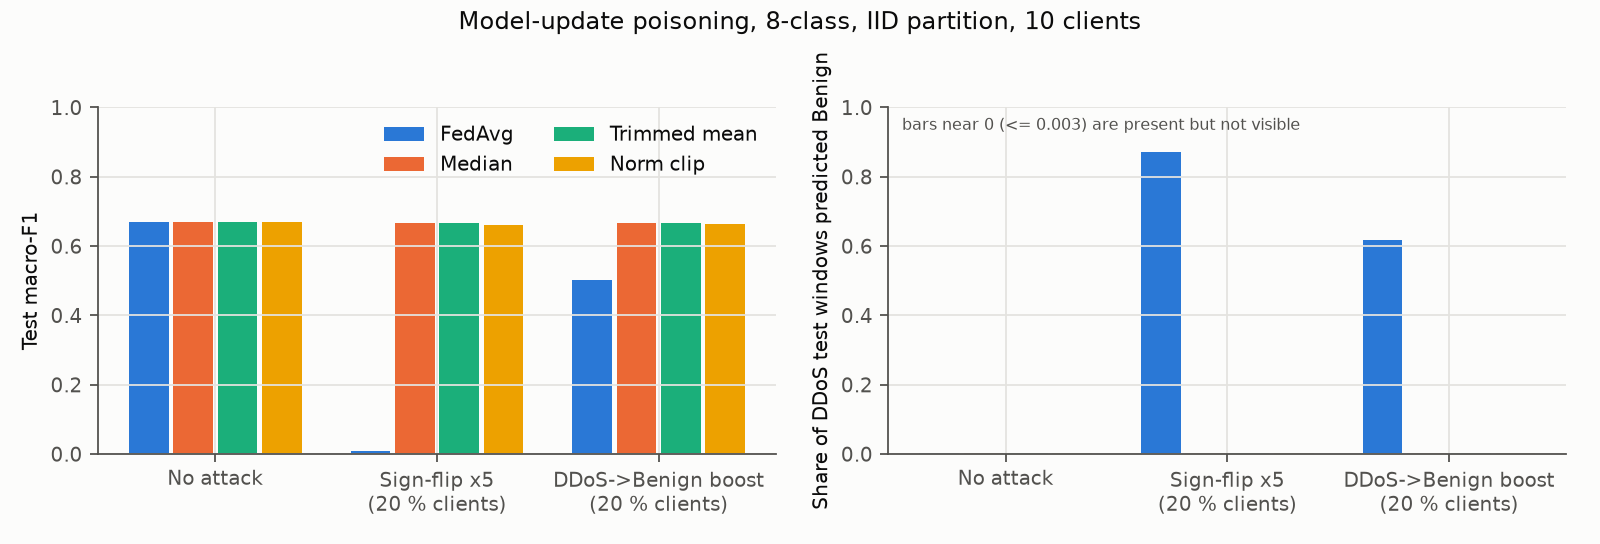
\includegraphics[width=\columnwidth]{m6_poisoning_category_iid.png}
\caption{Poisoning, 8-class, IID clients: macro-F1 (left) and share of DDoS windows predicted Benign (right) per aggregator.}
\label{fig:pois}
\end{figure}

\subsection{Evasion and adversarial training}
\textbf{Which families evade.} Flood families (DDoS, DoS, Mirai) are rarely evaded. Spoofing, Web, Recon and Brute force can be made to look benign 20--65\,\% of the time; these are the families already confused with Benign. Most successes need no slow-down.

\textbf{The deployable threshold is the most evadable.} At the 1\,\% threshold, the round-0 evasion rate is 1.1--2.1$\times$ the argmax rate: 0.24--0.41 for the v2 MLP and 0.33--0.49 for HGB. The binary RF looked robust at argmax (0.04), but only because it flagged 59\,\% of benign traffic. At a fixed FPR, every model is evadable.

\textbf{Adversarial training.} One round of adversarial training reduces evasion 2--3$\times$ in every task and model. After two rounds it is 0.09--0.12 for the MLP and 0.08--0.17 for HGB (Fig.~\ref{fig:adv}). Clean detection changes by $-0.011$ to $+0.005$, and the benign FPR stays at 0.9--1.25\,\%. Spoofing (0.28--0.69) and Web (0.20--0.50) remain evadable.

\begin{figure}[t]
\centering
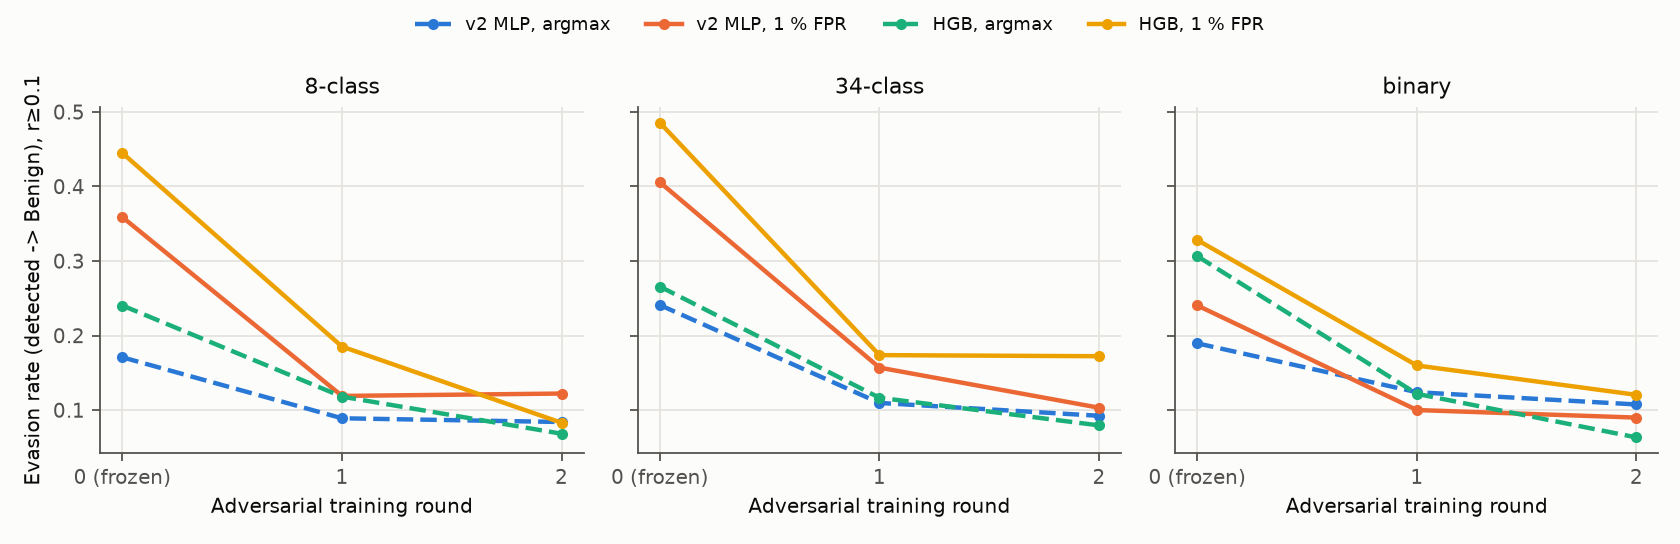
\includegraphics[width=\columnwidth]{wp5_advtrain_evasion.png}
\caption{Evasion rate ($r\ge0.1$) per adversarial-training round, at argmax and at the 1\,\%-FPR threshold.}
\label{fig:adv}
\end{figure}

\subsection{LLM-planned attacks}
\textbf{Results.} Leave-one-LLM-out volume features reach AUC 0.903--1.000 and detect every session. A one-line rule (``IP address with more than one source MAC'') flags 89--99\,\% of attack windows with no false alarms on held-out normal operation.

\textbf{Why the planner barely matters.} All sessions execute through the same toolkit (ARP MITM plus S7/Modbus modification), so the signature is set by the tools, not the LLM.

\textbf{Without the ARP signature.} Removing the ARP and host-count features lowers AUC by only 0.003--0.007, and 98--100\,\% of sessions are still found. The residual signal is the MITM relay itself: about 5\,\% more S7 packets per window. SCADA process data alone carry no usable signal in this form (AUC 0.37--0.58).

\section{Discussion and Limitations}
\textbf{What drove the results.} Data handling and the operating point, not model choice, determined the numbers. Each defence carries a measurable assumption that an attacker can step outside:
\begin{itemize}
\item calibration moves the threshold towards evadable territory;
\item robust aggregation assumes a bounded malicious fraction and mild heterogeneity;
\item adversarial training assumes a known perturbation space;
\item the GridStratLLM detection assumes a MITM step.
\end{itemize}

\textbf{Limitations.}
\begin{itemize}
\item One dataset release, one split and one hardware setup. The poisoning sweep and non-IID poisoning cells use one seed.
\item 17 of 34 classes are separated only in time.
\item Evasion is modelled in feature space and not replayed through the feature extractor. Adversarial training was tested only against the same attacker.
\item Multi-Krum, FLTrust and formal privacy were not evaluated.
\item Comparisons with prior work rest on their published tables, not their split files.
\end{itemize}

\section{Conclusion}
Under a leakage-aware protocol, CICIoT2023 multi-class detection is about 0.69 macro-F1, consistent with the dataset authors' benchmark and well below recent federated reports. A calibrated 1\,\% FPR operating point makes the detectors usable, but it is also where evasion is easiest. Adversarial training cuts evasion 2--3$\times$ at negligible clean cost.

Federated training matches centralised training under mild heterogeneity, and a real cross-cloud deployment reproduced the simulation exactly. Strong label skew remains unsolved. Robust aggregation stops two poisoning clients only within its assumptions. LLM-planned attacks on a smart-grid testbed are detectable because their signature is set by the attack toolkit.

Future work: adaptive attackers, clustered FL for label skew, multi-Krum and FLTrust under the same protocol, and replay of evasion through the feature extractor. Code, tests and run records are available at \url{https://github.com/vinitsoni03/federated-ids}.

\bibliographystyle{IEEEtran}
\bibliography{refs}

\end{document}
